\section{Experiments}

\setlength{\tabcolsep}{8pt}
% [ Check RGB-D single modality ]
\begin{table}[t]
\begin{center}
\vspace{3mm}
\caption{Top-1 \textit{mean} accuracy ($\%$) of different common-use architectures, over all $D_i \rightarrow D_j$ combinations on both seen and unseen test sets in \textit{offline-trimmed} setting. }
\label{tab:backbone}
\begin{tabular}{lccccc}%{lC{1.5cm}C{1.5cm}C{1.5cm}}
\toprule\noalign{\smallskip}
\multicolumn{5}{c}{\normalsize\textsc{EPIC-Kitchens 55}} \\
\noalign{\smallskip}
\cline{1-5}
\noalign{\smallskip}
Network  & Sampling & Params & Seen & Unseen \\
\noalign{\smallskip}
\toprule\noalign{\smallskip}
\multirow{1}{*}{\centering TSN} 
  & U 5x5 & 10.7M & 60.88 & 31.55 \\
 
  \noalign{\smallskip}

 \multirow{1}{*}{\centering TSN-TRN} 
  & U 5x5  & 18.3M & 63.13 & 32.42 \\
 

 \noalign{\smallskip}
\multirow{1}{*}{\centering TSM} 
  & U 5x5 &  24.3M & \textbf{71.48} & 35.97 \\
 
  
   \noalign{\smallskip}
\multirow{1}{*}{\centering TSM-TRN} 
  & U 5x5 & - & 69.52 & 36.05 \\
 
  \hline 
 \noalign{\smallskip}
\multirow{1}{*}{\centering I3D }
  & U 16x5 & 12.4M & 67.34 & \textbf{43.89} \\ 
 
 \noalign{\smallskip}
\multirow{1}{*}{\centering I3D }
  & D 16x5 & 12.4M & 67.08 & 42.42 \\
    \hline
 \noalign{\smallskip}
\multirow{1}{*}{\centering X3D-XS }
  & U 5x5 & 3.8M & 51.46 & 36.39 \\ 	

 \noalign{\smallskip}
\multirow{1}{*}{\centering X3D-XS }
  & D 16x5 & 3.8M & 48.45 & 32.66 \\
  

    \noalign{\smallskip}
\multirow{1}{*}{\centering MoViNet-A0 }
  & U 5x5 & 3.1M & \rev{62.17} & \rev{39.25} \\

  
     \noalign{\smallskip}
\multirow{1}{*}{\centering MoViNet-A0 }
  & D 16x5 & 3.1M & \rev{64.17} & \rev{40.68} \\

\bottomrule
\end{tabular}
\end{center}
\vspace{-5mm}
\end{table}
\setlength{\tabcolsep}{1.4pt}



\setlength{\tabcolsep}{7pt}
% [ Check RGB-D single modality ]
\begin{table}[t]
\begin{center}
\vspace{3mm}
\caption{Top-1 \textit{mean} accuracy ($\%$), over all $D_i \rightarrow D_j$ combinations on both seen and unseen test sets in both \textit{offline-trimmed} setting and \textit{streaming-trimmed} setting}
\label{tab:offlinevsstream}
\begin{tabular}{lccccc}%{lC{1.5cm}C{1.5cm}C{1.5cm}}
\toprule\noalign{\smallskip}
\multicolumn{5}{c}{\normalsize\textsc{EPIC-Kitchens 55}} \\
\noalign{\smallskip}
\cline{1-5}
\noalign{\smallskip}
Network & Mode & Sampling & Seen & Unseen \\

  \hline
 \noalign{\smallskip}
\multirow{1}{*}{\centering I3D  }
 & Offline  & D 16x5 & 67.08 & 42.42 \\
 
 
 \noalign{\smallskip}
\multirow{1}{*}{\centering X3D-XS  }
 & Offline  & D 16x5 & 48.45 & 32.66 \\


 \noalign{\smallskip}
\multirow{1}{*}{\centering MoViNet-A0  }
 & Offline  & D 16x5 & \rev{64.17} & \rev{40.68} \\

\hline

 \noalign{\smallskip}
\multirow{1}{*}{\centering I3D  }
 & Streaming & All Stream & \textbf{63.38} & \textbf{40.57} \\
 

 \noalign{\smallskip}
\multirow{1}{*}{\centering X3D-XS  }
 & Streaming & All Stream & 43.37 & 32.31 \\
 	
  
 \noalign{\smallskip}
\multirow{1}{*}{\centering MoViNet-A0  }
 & Streaming & All Stream & 62.24 & 39.59 \\

\bottomrule
\end{tabular}
\end{center}
\vspace{-5.5mm}
\end{table}

\setlength{\tabcolsep}{1.4pt}

\textbf{Backbones comparisons. } 
%In Table %\ref{tab:netsize} we compare different commonly known architectures adopted in action recognition with more recently NAS-based compressed models. We regrouped them in 2D based ones, such as TSN, TSM and TRN and 3D models (I3D, X3D and MoViNet). From this first distinction it is possible to observe how different aspects, such as different pretrain, sampling and model size, influence the performance on a strongly motion-based and fine-grained dataset. Uniform sampling usually produces better results, which is to be expected because it allows you to span across the entire video without forwarding all frames. %Such a sampling strategy is crucial for 2D architectures to model motion properly. 
%Unfortunately, it is based on the strong assumption that the action has already been completed and that you know the activity's boundaries (start and finish), which limits its use in an online setting.
%Indeed, the temporal stride adopted for such a sampling strategy is dynamic and dependant on the length of the sample. 
%Another important analysis which should be considered is the cross-domain one. In fact, it allows us to observe decrease in accuracy caused by the different data distribution in each model. This kind of situation generates understanding on how the model really behaves in real world scenario and, secondary, a recent studio \cite{plizzari2022e2} highlight a strong correlation between the decrease of performance in unseen scenario and  how much the network suffers to encode appearance information instead of motion one. Despite performing well on \textit{seen} situations, 2D models obtain a bigger gap in performance on \textit{unseen} ones making them strongly dependent on the training data and not suitable for realistic scenarios. 
%Due to those considerations, we shift our focus towards 3D based architectures. Among those, I3D remains the best performing model under dense sampling conditions but at a much higher cost in terms of parameters. Finally, when comparing the two smaller models (MoViNet-A0 and X3D-XS), MoViNet appears to be the better choice; it achieves higher results in both seen and unseen results and it is more resistant to the change in sampling passing from U$\rightarrow$D.
In Table \ref{tab:backbone} we compare different commonly known architectures adopted in action recognition taking in consideration different aspects, such as: 2D and 3D base models, different pretrains, sampling strategies and numbers of params, observing how all this characteristics impact the performances in both seen and unseen scenario. 
We regrouped them into 2D-based (TSN, TSM, and TRN) and 3D-based (I3D, X3D, and MoViNet). From this first distinction, it is possible to observe how a pure 2D convolution as in TSN, without any temporal modeling, achieves lower performance compared to the other 2D models, in particular in unseen scenarios. We can observe from Table \ref{tab:backbone} that, by increasing the capacity of the model to encode the temporal information, we obtain an improvement equal to 3$\%$ and 1$\%$, using the temporal relation module (TRM). Using an architecture with the capacity to encode temporal information, such as TSM, the improvement with respect to the TSN performance is equal to 11 and 4 in the seen and unseen scenarios. We further observe that the temporal shift module used in TSM to encode the temporal information, a mechanism based on a partial shift among the channels of the adjacent frames, is enough for the respective 2D architecture to encode the motion information. In fact, enriching the model with a TRN module does not obtain the same improvement as in the TSN model. The second important aspect that we can observe from this first group of experiments is related the drastically decrease of the performance of the model when the training and test data do not share the same distribution. %This issue, known as environmental bias, originates from networks’ tendency to rely on the environment in which activities are recorded. It affects their ability to recognize actions when they are performed in unfamiliar (unseen) surroundings, resulting in a performance decline equal to half the final performance.
This problem, known as environmental bias, causes a performance drop equivalent to half of the final performance. This is mainly caused by 2D based (appearance-based) networks’ tendency to primarily focus on background cues and objects texture, which are typically uncorrelated with the action being performed and thus largely varying in different environments.

Moving towards the second group of experiments, based on 3D convolution, we can notice the different pretrains due to the fact that the 3D convolution used to encode both spatial and temporal dimensions needs a pretrain on a large scale video dataset, such as Kinetics. The second important aspect that it is easy to notice is that the performances in the seen scenario seem to be lower compared with the previous 2D-CNN group. The best result is the 62.45$\%$ of MoViNet w.r.t. the 71.48$\%$ of TSM (same configurations). We believe that the unseen scenario is helpful to avoid being fooled by these results and it allows us to reconsider this second group comparable with the first one. Indeed, the performance in the unseen scenario is comparable and, in some cases, better w.r.t. the 2D-CNN. We believe that this behavior is due to the tendency of the 2D-CNNs to overfit by leveraging domain-specific features more with respect to the 3D-CNNs.

Another factor to consider is the sampling strategy. In the literature, 2D-CNN is frequently trained with a uniform strategy, and X3D and MoViNet appear to benefit more from dense sampling than I3D. This is because their own pretrain on Kinetics (unlike I3D) is made with a very large stride (12 for X3D and 6 for MoViNet) that is closer to a uniform solution than the standard dense solution that has stride 2 for 60 fps videos (equal to 1 with 30 fps). 

%In general, uniform solutilon allows for better performance by allowing all video to be encoded with fewer frames (reducing redundancy). Ideally, for the dense solution, we should pass all or the majority of the frames of the video together, but the limited memory size makes it an infeasible approach. Considering this limitation, a standard solution is to use during test five short clips of 16 frames each, which are passed into the model and the corresponding outputs combined to obtain a video level prediction. The limited clip size w.r.t the whole video length is a strong limitation for the model to learn a good representation of the action. Indeed, by switching from 16 dense frames to 5 uniform ones, X3D and MoViNet improved by 8$\%$-5$\%$ and 10$\%$-2.5$\%$, respectively, for both scenarios.

Unfortunately, this strategies is based on the strong assumption that the action has already been completed and that you know the activity's boundaries (start and finish), which limits its use in an online setting. Indeed, the temporal stride adopted for such a sampling strategy is dynamic and dependent on the length of each sample. Due to those considerations, we shift our focus towards 3D based architectures. Among those, I3D remains the best performing model under dense sampling conditions, obtaining a gap up to 5$\%$ and 1$\%$ w.r.t MoViNet and 14$\%$ and 5$\%$ w.r.t X3D.   

\textit{How impact the model size on the final performances?} Due to their lower model sizes, MoViNet and X3D were included in our benchmark in order to understand how the smaller model size influences the final performance of the model. In the case of X3D, the tiny model size appears to have an impact on the final results; in fact, it provides the lowest results. It also appears to suffer greatly from the transition from uniform to dense sampling (U$\rightarrow$D). MoViNet, on the other hand, appears to be the preferable alternative; it generates greater results in both seen and unseen outcomes and is more resistant to the shift in sample going from uniform to dense (U$\rightarrow$D). For these reasons, we pay special attention to this network in our work.


\begin{comment}

\begin{itemize}
    \item In table 1, we can see the comparison of popular action recognition architectures. We regroup in 2D based, as .. and 3D based...
    From these comparisons emerged other important aspects, such as different pretrain, different sampling, and model size.
    \item The value of cross-domain analysis may be observed not only in the decrease in accuracy caused by the different data distribution in each model, but also in how the unknown situation helps us to understand the true behavior of the model, as in the case of TSM and i3D.

    \item We reported the top-1 accuracy for both seen and unseen scenario following the offline action recognition scenario with trimmed videos.
    \item When comparing the two smaller models (MoViNet and X3D-XS), MoViNet appears to be the better choice; it achieves higher results in both seen and unseen results when compared to the X3D-XS. They appear to be more resistant to the change in sampling passing from U->D.
    
\end{itemize}
\end{comment}

\textbf{Passing from offline to streaming.} %Proceeding in our analysis, we shifted our focus from a purely offline setting, where the models know what are the frames of the video and sample them in the most suited manner for the model, to a streaming version which is closer to reality. Indeed, it is expected that deployed architectures are able to perform inference on a stream of frames which are sampled at a fixed temporal resolution, i.e. densely sampled. The results in this different context are reported in Table \ref{tab:offlinevsstream}. In particular, it is important to mention that, among the state-of-the-art models in action recognition, MoViNet is the only architecture that takes into account directly the possibility to keep information about the past thanks to the streaming buffer mechanism. Differently, the other 3D models, require the adoption of late fusion techniques of logits in order to properly process the video stream. In particular, to fit these models to a continuous stream of frames we generated artificial clips by concatenating the current input frame with the past 15 and we averaged the logits for all the frames of the sample. For simplicity, from now on, we will denote this "online adaptation" for 3D models as \textit{accumulation strategy}. Despite being computationally more extensive, the performance obtained trough this technique are on-par with the one of MoViNet as soon as 30\% of the video is observed and they barely improve. Instead, with the help of the streaming buffer MoViNet model is able to perform inference on a single frame per time and increase rapidly the knowledge about the past making it perfectly suitable for this situation.
%In Table \ref{tab:backbone}, we differentiate between sampling strategies (uniform and dense) and which one is more adaptable to realistic scenarios. However, both solutions must be considered "offline" 
%because they are applied to a subsample of the entire sample. %based on prior knowledge on the beginning and end of the video to guide the sampling. We take equidistant frames with uniform sampling, and multiple equidistant clips are picked in the dense solution to obtain video level prediction.
In a real-world scenario, a wearable device should be able to deal with a continuous stream of data. In this section, we want to study how a model behaves when passing from an offline setting, where the standard action recognition methods usually work, to a new one, called streaming, where all the video is fed as input to the model in a "continuous" fashion, obtaining a continuous output. 
%For this new scenario, we have to make a distinction between the behavior of the architectures works. As regards I3D and X3D, we extended the offline technique based on the averaging of five clips' output to averaging a continuous output obtained by shifting a temporal window along the whole video and forwarding a continuous updating clip at the network's input. The updating clip consists of adding a new frame accumulated with the oldest stored frames after deleting the oldest one. Unlike the previous two, MoViNet already has its own streaming version, which replaces 3D convolution with the (2+1)D operation and exposes a stream buffer mechanism to cache feature activations, allowing to expand the temporal receptive field without the need of recomputation, as in I3D or X3D. To support frame-by-frame output and exploit the buffer mechanism, it uses the Causal Convolutions, making them unidirectional along the temporal dimension, and Cumulative Global Average Pooling,  to approximate any global average pooling involving the temporal dimension.
Table \ref{tab:offlinevsstream} shows the results in this distinct setting. It is especially clear that MoViNet is the only network that benefits from seeing complete video, as opposed to the other two models, which achieve a minimal variation in performance. The MoViNet’s improvement is significant, with increases of up to 10\% and 4\% in seen and unseen scenarios, respectively.Furthermore, I3D and X3D using for each output $T_{s}$ dense frame with $T_{s}$ equal to 16 means, it implies that they requires to recompute frame activations which overlap, reducing the efficiency 





\begin{figure}[t!]
\vspace{2mm}
\centering
\hspace{-15px}
\begin{minipage}[t]{\columnwidth}
 %   \subfloat[]{
     \resizebox {\columnwidth} {!} {
        \begin{tikzpicture}
        \pgfplotsset{every axis legend/.append style={
at={(0.5,1.03)},
anchor=south}}

        % LEFT AXIS
        % =========
        \begin{axis}[
          enlargelimits=false,
          ylabel={Top-1 Accuracy (\%)},
          xlabel={Percentage (\%)},
           xmin=0, xmax=100,
           ymin=26, ymax=68,
          xtick={0,20,40,60,80,100},
          ytick={30,40,50,60},
          %legend pos=south west,
          xmajorgrids=true,
          ymajorgrids=true,
          grid style=dashed,
          width=15cm,
          height=8cm,
          legend columns=3,
          legend style={font=\LARGE},
          label style={font=\LARGE},
          tick label style={font=\LARGE},
        legend style={draw=none},
        every axis plot/.append style={ultra thick},
        every mark/.append style={mark size=50pt}
        ]
        
        \addplot[
          color=MaterialBlue800]
        table[x index=0,y index=1,col sep=comma]
        {tex/Tables/Tab/I3D_full_sup.txt};
               \addlegendentry{I3D-(seen)} 
               
               
       \addplot[
          color=MaterialOrange800]
        table[x index=0,y index=1,col sep=comma]
        {tex/Tables/Tab/movinet_sup.txt};
               \addlegendentry{MoViNet-(seen)} 
               
        \addplot[
          color=greeno]
        table[x index=0,y index=1,col sep=comma]
        {tex/Tables/Tab/X3D_sup.txt};
               \addlegendentry{X3D-(seen)} 

         
       % \addlegendentry{Single-DG-RNA} 
        
        
        % An \addplot for each line
        \addplot[
          color=MaterialBlue800, dashed]
        table[x index=0,y index=1,col sep=comma]
        {tex/Tables/Tab/I3D_full_cross.txt};
       \addlegendentry{I3D-(unseen)} 


         
       % \addlegendentry{Single-DG-RNA} 
        
        
        % An \addplot for each line
        \addplot[
          color=MaterialOrange800, dashed]
        table[x index=0,y index=1,col sep=comma]
        {tex/Tables/Tab/movinet_cross.txt};
       \addlegendentry{MoViNet-(unseen)}
      
         
       % \addlegendentry{Single-DG-RNA} 
        
        
        % An \addplot for each line
        \addplot[
          color=greeno, dashed]
        table[x index=0,y index=1,col sep=comma]
        {tex/Tables/Tab/X3D_cross.txt};
       \addlegendentry{X3D-(unseen)} 

        \end{axis}
        
        \end{tikzpicture}%
      }

    \end{minipage}

\caption{MoViNet, X3D and I3D performance with respect to the percentage of video observed}
\vspace{-0.4cm}
\label{fig:videoperc}
\end{figure}

\begin{figure}[t!]
\centering
\begin{minipage}[t]{0.44\textwidth}
 %   \subfloat[]{
     \resizebox {\columnwidth} {!} {
        \begin{tikzpicture}
        \pgfplotsset{every axis legend/.append style={
at={(0.5,1.03)},
anchor=south}}

        % LEFT AXIS
        % =========
        \begin{axis}[
          enlargelimits=false,
          ylabel={\large  Seen Acc. (\%)},
          xlabel={},
           xmin=0, xmax=72,
           ymin=22, ymax=53,
          xtick={0,8,16,32,48,64},
          ytick={20,25,30,35,40,45,50},
          %legend pos=south west,
          ymajorgrids=true,
          grid style=dashed,
          width=10cm,
          height=4.5cm,
          legend columns=2,
        legend style={draw=none},
        every axis plot/.append style={ultra thick},
        every mark/.append style={mark size=50pt}
        ]
        
        \addplot[
          color=MaterialBlue800,
          mark=square*]
        table[x index=0,y index=1,col sep=comma]
        {tex/Tables/Tab/seen-clean-static-i3d.txt};
               \addlegendentry{I3D-(with clean)} 
         
        
        
        % An \addplot for each line
        \addplot[
          color=MaterialOrange800,
          mark=oplus*]
        table[x index=0,y index=1,col sep=comma]
        {tex/Tables/Tab/seen-clean-static-MoViNet.txt};
       \addlegendentry{MoViNet-(with clean)} 
       
       %%%%%%%%%%%%%%%%%%%%
       %  no clean buffer %
       %%%%%%%%%%%%%%%%%%%%
       
        \addplot[dotted,
          color=MaterialBlue800,]
        table[x index=0,y index=1,col sep=comma]
        {tex/Tables/Tab/seen-noclean-i3d.txt};
               \addlegendentry{I3D-(w/o clean)} 
         
        
        
        % An \addplot for each line
        \addplot[dotted,
          color=MaterialOrange800,]
        table[x index=0,y index=1,col sep=comma]
        {tex/Tables/Tab/seen-noclean-MoViNet.txt};
       \addlegendentry{MoViNet-(w/o clean)} 


        \end{axis}
        
        \end{tikzpicture}%
      }

    \end{minipage}
\begin{minipage}[t]{0.44\textwidth}
 %   \subfloat[]{
     \resizebox {\columnwidth} {!} {
        \begin{tikzpicture}
        \pgfplotsset{every axis legend/.append style={
at={(0.5,1.03)},
anchor=south}}

        % LEFT AXIS
        % =========
        \begin{axis}[
          enlargelimits=false,
          ylabel={\large Unseen Acc. (\%)},
          xlabel={},
           xmin=0, xmax=72,
           ymin=20, ymax=37,
          xtick={0,8,16,32,48,64},
          ytick={22,24,28,30,32,34},
          %legend pos=south west,
          ymajorgrids=true,
          grid style=dashed,
          width=10cm,
          height=4.5cm,
          legend columns=2,
        legend style={draw=none},
        every axis plot/.append style={ultra thick},
        every mark/.append style={mark size=50pt}
        ]
        
        \addplot[
          color=MaterialBlue800,
          mark=square*]
        table[x index=0,y index=1,col sep=comma]
        {tex/Tables/Tab/unseen-clean-static-i3d.txt};
               \addlegendentry{I3D-(with clean)} 

         
       % \addlegendentry{Single-DG-RNA} 
        
        
        % An \addplot for each line
        \addplot[
          color=MaterialOrange800,
          mark=oplus*]
        table[x index=0,y index=1,col sep=comma]
        {tex/Tables/Tab/unseen-clean-static-MoViNet.txt};
       \addlegendentry{MoViNet-(with clean)} 
        
        
       %%%%%%%%%%%%%%%%%%%%
       %  no clean buffer %
       %%%%%%%%%%%%%%%%%%%%
       
        \addplot[dotted,
          color=MaterialBlue800,]
        table[x index=0,y index=1,col sep=comma]
        {tex/Tables/Tab/unseen-noclean-i3d.txt};
               \addlegendentry{I3D-(w/o clean)} 
         
        
        
        % An \addplot for each line
        \addplot[dotted,
          color=MaterialOrange800,]
        table[x index=0,y index=1,col sep=comma]
        {tex/Tables/Tab/unseen-noclean-MoViNet.txt};
       \addlegendentry{MoViNet-(w/o clean)} 
        
        \end{axis}  
        
        \end{tikzpicture}%
      }

    \end{minipage}
%%%%%%%%%%%%%
%   graph   %
%%%%%%%%%%%%%

%\begin{minipage}[t]{0.44\textwidth}
 %   \subfloat[]{
%    \resizebox {\columnwidth} {!}{
%    \centering
%    %%%%%%%%%%%%%%%%%%%%%%%%%%%%%%%%%%%%%%%%%%%%%%%%%%%%%%%%%%%%%%%
%
% Welcome to Overleaf --- just edit your LaTeX on the left,
% and we'll compile it for you on the right. If you open the
% 'Share' menu, you can invite other users to edit at the same
% time. See www.overleaf.com/learn for more info. Enjoy!
%
%%%%%%%%%%%%%%%%%%%%%%%%%%%%%%%%%%%%%%%%%%%%%%%%%%%%%%%%%%%%%%%
%\usepgfplotslibrary{external}
%\tikzexternalize

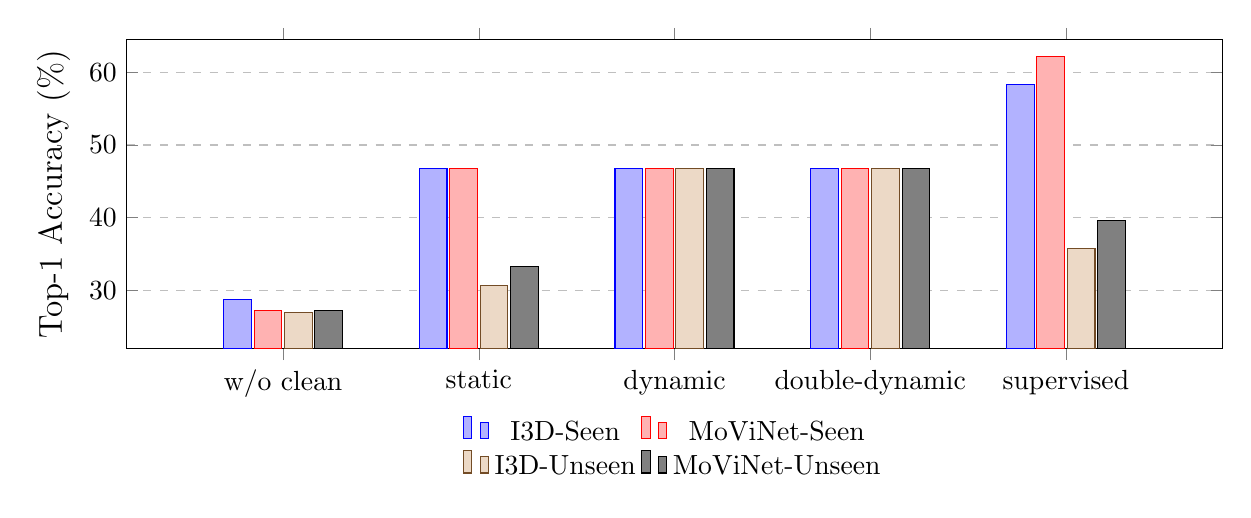
\begin{tikzpicture}
\centering
\begin{axis}[
symbolic x coords={w/o clean, static, dynamic, double-dynamic, supervised},
	ylabel=\large Top-1 Accuracy (\%),
	enlargelimits=false,
	ybar=1pt, enlarge x limits=0.2,
	xtick=data,
	ymin=22.0,
    ymax=64.5,
    ymajorgrids=true,
    legend style={draw=none},
          grid style=dashed,
          width=15.5cm,
          height=5.5cm,
         legend style={at={(0.5,-0.2)},
	    anchor=north,legend columns=2}, 
        every axis plot/.append 
        every mark/.append style={mark size=52pt}
]
\addplot 
	coordinates {(w/o clean,28.73) (static,46.77) (dynamic,46.77) (double-dynamic,46.77)
	(supervised,58.33) };
	\addlegendentry{I3D-Seen} 
\addplot 
	coordinates {(w/o clean,27.20) (static,46.71) (dynamic,46.71)(double-dynamic,46.77)
	(supervised,62.24) };
	\addlegendentry{MoViNet-Seen} 
\addplot 
	coordinates {(w/o clean,26.96) (static,30.71) (dynamic,46.71)(double-dynamic,46.77)
	(supervised,35.71) };
\addlegendentry{I3D-Unseen} 
\addplot 
	coordinates {(w/o clean,27.20) (static,33.30) (dynamic,46.71)(double-dynamic,46.77)
	(supervised,39.59) };
\addlegendentry{MoViNet-Unseen} 

\end{axis}
\end{tikzpicture}



%    }
%    \vspace{0.4cm}
%    \end{minipage}    


%%%%%%%%%%%%%%
%   graph 2  %
%%%%%%%%%%%%%%
%\begin{minipage}[t]{0.44\textwidth}
% %   \subfloat[]{
%    \resizebox {\columnwidth} {!}{
%    \centering
%    %%%%%%%%%%%%%%%%%%%%%%%%%%%%%%%%%%%%%%%%%%%%%%%%%%%%%%%%%%%%%%%
%
% Welcome to Overleaf --- just edit your LaTeX on the left,
% and we'll compile it for you on the right. If you open the
% 'Share' menu, you can invite other users to edit at the same
% time. See www.overleaf.com/learn for more info. Enjoy!
%
%%%%%%%%%%%%%%%%%%%%%%%%%%%%%%%%%%%%%%%%%%%%%%%%%%%%%%%%%%%%%%%
%\usepgfplotslibrary{external}
%\tikzexternalize

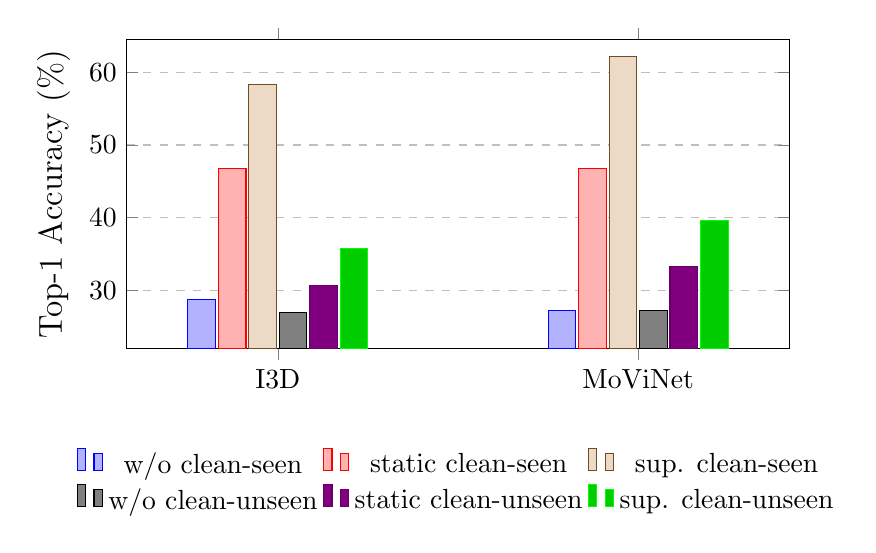
\begin{tikzpicture}
\begin{axis}[
symbolic x coords={I3D, MoViNet},
	ylabel=\large Top-1 Accuracy (\%),
	enlargelimits=false,
	ybar=1pt, enlarge x limits=0.42,
	xtick=data,
	ymin=22.0,
    ymax=64.5,
    ymajorgrids=true,
    legend style={draw=none},
          grid style=dashed,
          width=10cm,
          height=5.5cm,
         legend style={at={(0.5,-0.3)},
	    anchor=north,legend columns=3}, 
        every axis plot/.append 
        every mark/.append style={mark size=52pt}
]
\addplot 
	coordinates {
	            (I3D,28.73)
	            (MoViNet,27.20)
	};
	\addlegendentry{w/o clean-seen} 
\addplot 
	coordinates {
	            (I3D,46.77)
	            (MoViNet,46.71)
	};
	\addlegendentry{static clean-seen} 
\addplot 
	coordinates {
	            (I3D,58.33)
	            (MoViNet,62.24)
	};
	\addlegendentry{sup. clean-seen} 
	
	
	

\addplot 
	coordinates {
	            (I3D,26.96)
	            (MoViNet,27.20)
	};
	\addlegendentry{w/o clean-unseen} 

\addplot 
	coordinates {
	            (I3D,30.71)
	            (MoViNet,33.30)
	};
	\addlegendentry{static clean-unseen} 

\addplot 
	coordinates {
	            (I3D,35.71)
	            (MoViNet,39.59)
	};
	\addlegendentry{sup. clean-unseen} 

\end{axis}
\end{tikzpicture}



%    }
%    
%    \end{minipage}    
        
    

\caption{\textbf{Static boundary localization.} Top-1 \textit{mean} accuracy ($\%$), over all $D_i \rightarrow D_j$ combinations on both seen (up) and unseen (down) test sets in \textit{online-trimmed} setting, with different clean buffer strategy w.r.t the no-clean buffer. }
\label{fig:clean_static}
\end{figure}

\begin{figure}[t!]
\centering
\begin{minipage}[t]{0.44\textwidth}
 %   \subfloat[]{
     \resizebox {\columnwidth} {!} {
        \begin{tikzpicture}
        \pgfplotsset{every axis legend/.append style={
at={(0.5,1.03)},
anchor=south}}


        % LEFT AXIS
        % =========
        \begin{axis}[
          enlargelimits=false,
          ylabel={\large Seen Acc. (\%)},
          xlabel={},
           ymin=38.5, ymax=56,
           xmin=0.2, xmax=1.1,
          xtick={0.3,0.4,0.5,0.6,1},
          ytick={40,42,45,50,53},
          %legend pos=south west,
          ymajorgrids=true,
          grid style=dashed,
          width=10cm,
          height=4.5cm,
          legend columns=2,
        legend style={draw=none},
        every axis plot/.append style={ultra thick},
        every mark/.append style={mark size=50pt}
        ]
        
        \addplot[
          color=MaterialBlue800,
          mark=square*]
        table[x index=0,y index=1,col sep=comma]
        {tex/Tables/Tab/seen-clean-dynamically-i3d.txt};
               \addlegendentry{I3D dynamic} 

         
       % \addlegendentry{Single-DG-RNA} 
        
        
        % An \addplot for each line
        \addplot[
          color=MaterialOrange800,
          mark=oplus*]
        table[x index=0,y index=1,col sep=comma]
        {tex/Tables/Tab/seen-clean-dynamically-MoViNet.txt};
       \addlegendentry{MoViNet dynamic} 
        
    \addplot[dotted,
          color=MaterialBlue800,
          mark=triangle]
        table[x index=0,y index=1,col sep=comma]
        {tex/Tables/Tab/clean-statically-i3d-seen.txt};
       \addlegendentry{I3D static} 
      
      \addplot[dotted,
          color=MaterialOrange800,
          mark=triangle]
        table[x index=0,y index=1,col sep=comma]
        {tex/Tables/Tab/clean-statically-MoViNet-seen.txt};
       \addlegendentry{MoViNet static} 
    
        
        
        \end{axis}
        
        \end{tikzpicture}%
      }

    \end{minipage}

\begin{minipage}[t]{0.44\textwidth}
 %   \subfloat[]{
    \vspace{0.4cm}
     \resizebox {\columnwidth} {!} {
        \begin{tikzpicture}
        \pgfplotsset{every axis legend/.append style={
at={(0.5,1.03)},
anchor=south}}

        % LEFT AXIS
        % =========
        \begin{axis}[
          enlargelimits=false,
          ylabel={\large Unseen Acc. (\%)},
          xlabel={},
           xmin=0.2, xmax=1.1,
           ymin=28, ymax=37,
          xtick={0.3,0.4,0.5,0.6,1},
          ytick={22,24,28,30,32,34,36},
          %legend pos=south west,
          ymajorgrids=true,
          grid style=dashed,
          width=10cm,
          height=4.5cm,
          legend columns=2,
        legend style={draw=none},
        every axis plot/.append style={ultra thick},
        every mark/.append style={mark size=50pt}
        ]
        
        \addplot[
          color=MaterialBlue800,
          mark=square*]
        table[x index=0,y index=1,col sep=comma]
        {tex/Tables/Tab/unseen-clean-dynamically-i3d.txt};
        \addlegendentry{I3D dynamic} 

         
       % \addlegendentry{Single-DG-RNA} 
        
        
        % An \addplot for each line
        \addplot[
          color=MaterialOrange800,
          mark=oplus*]
        table[x index=0,y index=1,col sep=comma]
        {tex/Tables/Tab/unseen-clean-dynamically-MoViNet.txt};
       \addlegendentry{MoViNet dynamic} 
       
       \addplot[dotted,
          color=MaterialBlue800,
          mark=triangle]
        table[x index=0,y index=1,col sep=comma]
        {tex/Tables/Tab/clean-statically-i3d-unseen.txt};
       \addlegendentry{I3D static} 
      
      \addplot[dotted,
          color=MaterialOrange800,
          mark=triangle]
        table[x inde x=0,y index=1,col sep=comma]
        {tex/Tables/Tab/clean-statically-MoViNet-unseen.txt};
       \addlegendentry{MoViNet static} 
       
       
       
       
        \end{axis}

        \end{tikzpicture}%
      }

    \end{minipage}
    
\caption{\textbf{Dynamic boundary localization.} Top-1 \textit{mean} accuracy ($\%$), over all $D_i \rightarrow D_j$ combinations on both seen (up) and unseen (down) test sets in \textit{online-trimmed} setting, with different threshold-values. }
\label{fig:dynamically_clean}
\end{figure}
\begin{figure}[t!]
\centering
\begin{minipage}[t]{0.23\textwidth}
   \resizebox {\columnwidth} {!}{
    \centering
    %%%%%%%%%%%%%%%%%%%%%%%%%%%%%%%%%%%%%%%%%%%%%%%%%%%%%%%%%%%%%%%
%
% Welcome to Overleaf --- just edit your LaTeX on the left,
% and we'll compile it for you on the right. If you open the
% 'Share' menu, you can invite other users to edit at the same
% time. See www.overleaf.com/learn for more info. Enjoy!
%
%%%%%%%%%%%%%%%%%%%%%%%%%%%%%%%%%%%%%%%%%%%%%%%%%%%%%%%%%%%%%%%
%\usepgfplotslibrary{external}
%\tikzexternalize


\begin{tikzpicture}
\centering
\begin{axis}[
symbolic x coords={\cite{du2022fast}, $A$, \textbf{$A^{2}$}, \textcolor{battleshipgrey}{S}},
	ylabel= Seen Acc. (\%),
	enlargelimits=false,
	ybar=0.5pt, enlarge x limits=0.15,
	xtick=data,
	ymin=28.0,
    ymax=66,
    ymajorgrids=true,
    legend style={draw=none},
          grid style=dashed,
          width=5.9cm,
          height=5cm,
         legend style={at={(0.5,-0.28)},
	    anchor=north,legend columns=2}, 
        every mark/.append style={mark size=7pt}
]
\addplot [fill=MaterialBlue600,]
	coordinates {
	(\cite{du2022fast},50.1)
	($A$,52.4)
	(\textbf{$A^{2}$},60.38)
	(\textcolor{battleshipgrey}{S},64.03)
	};
\addlegendentry{I3D} 

\addplot [fill=MaterialOrange600,]
	coordinates {
	(\cite{du2022fast},44.61)
	($A$,48.17 )
	(\textbf{$A^{2}$},52.87)
(\textcolor{battleshipgrey}{S},55.6)
	};
\addlegendentry{MoViNet} 


\end{axis}

\end{tikzpicture}





    }
    \vspace{-0.9cm}
\end{minipage}    
\begin{minipage}[t]{0.23\textwidth}
   \resizebox {\columnwidth} {!}{
    \centering
    %%%%%%%%%%%%%%%%%%%%%%%%%%%%%%%%%%%%%%%%%%%%%%%%%%%%%%%%%%%%%%%
%
% Welcome to Overleaf --- just edit your LaTeX on the left,
% and we'll compile it for you on the right. If you open the
% 'Share' menu, you can invite other users to edit at the same
% time. See www.overleaf.com/learn for more info. Enjoy!
%
%%%%%%%%%%%%%%%%%%%%%%%%%%%%%%%%%%%%%%%%%%%%%%%%%%%%%%%%%%%%%%%
%\usepgfplotslibrary{external}
%\tikzexternalize

\begin{tikzpicture}
\centering
\begin{axis}[
symbolic x coords={\cite{du2022fast}, $A$, \textbf{$A^{2}$}, \textcolor{battleshipgrey}{S}},
		ylabel= Unseen Acc. (\%),
	enlargelimits=false,
	ybar=0.5pt, enlarge x limits=0.15,
	xtick=data,
	ymin=22.0,
    ymax=42,
    ymajorgrids=true,
    legend style={draw=none},
          grid style=dashed,
            width=5.9cm,
          height=5cm,
         legend style={at={(0.5,-0.28)},
	    anchor=north,legend columns=2}, 
        every axis plot/.append 
        every mark/.append style={mark size=7pt}
]

\addplot [fill=MaterialBlue600,]
	coordinates {
	(\cite{du2022fast},36.74)
	($A$,36.12)
	(\textbf{$A^{2}$},39.28)
	(\textcolor{battleshipgrey}{S},40.57)
	};
\addlegendentry{I3D}


\addplot [fill=MaterialOrange600,]
	coordinates {
	(\cite{du2022fast},32.88)
	($A$,32.51 )
	(\textbf{$A^{2}$},35.19)
	(\textcolor{battleshipgrey}{S},37) };
\addlegendentry{MoViNet} 

\end{axis}
\end{tikzpicture}



    }
    \vspace{-1.4cm}
\end{minipage}    
\caption{ Top-1 \textit{mean} accuracy ($\%$), over all $D_i \rightarrow D_j$ combinations on both seen (left) and unseen (right) test sets in \textit{online-untrimmed} setting, using ABD\cite{du2022fast} to find the boundaries as secondary stream, our DBL technique with single aggregator ($A$) and with twofold aggregator  (\textbf{$A^{2}$}). The streaming (\textcolor{battleshipgrey}{S}) results are reported as upper bound reference.}
\label{fig:final_results}
\vspace{-0.5cm}
\end{figure}
    


\setlength{\tabcolsep}{2.0pt}

\begin{table}[t]
\vspace{3mm}
\begin{center}

\caption{MACs, FPS (Hz), Latency (ms, \rev{inference time}) and Energy(watt) on different devices.}
\label{tab:device}
\begin{tabular}{lccccc}%{lC{1.5cm}C{1.5cm}C{1.5cm}}
\toprule\noalign{\smallskip}
\multicolumn{6}{c}{\normalsize\textsc{On Device}} \\
\noalign{\smallskip}
\cline{1-6}
\noalign{\smallskip} 
Network & Device & MACs & FPS & Lat.(ms) & Power(watt) \\
\hline
\noalign{\smallskip}
\multirow{1}{*}{\centering I3D }
 &  2080 Ti  & \rev{$270e^8$} & 110 & $9.1$ & 53.7  \\
\multirow{1}{*}{\centering MoViNet }
 &  2080 Ti  & $0.47e^8$ & 781 & $1.3$  &  52 \\
% \multirow{1}{*}{\centering MoViNet** }
% & Titan RTX  &  &  & $44.6\pm 0.6$ &  \\
 \hline
\noalign{\smallskip}
\multirow{1}{*}{\centering I3D }
 &   MX350 & \rev{$270e^8$} & \textcolor{red}{\textbf{15}} & $65.7$ & 24.9  \\
\multirow{1}{*}{\centering MoViNet }
 &   MX350 & $0.47e^8$ & 169 & $5.9$  & 11.5 \\
% \multirow{1}{*}{\centering MoViNet** }
% & 2080 Ti  &  &  & $15.3\pm 0.2$ &  \\
 \hline
\noalign{\smallskip}
\multirow{1}{*}{\centering I3D } 
&   Jetson Nano  & \rev{$270e^8$} & \textcolor{red}{\textbf{3}} & $393.7$ & 3.7 \\
\multirow{1}{*}{\centering MoViNet }
 &  Jetson Nano  & $0.47e^8$ & \textcolor[rgb]{0,0.502,0}{\textbf{56}} &  $17.9$ & \textcolor[rgb]{0,0.502,0}{\textbf{2.4}}  \\
% \multirow{1}{*}{\centering MoViNet** }
% & Jetson Nano &  &  & $165\pm 7$ &  \\
\bottomrule
\end{tabular}
\end{center}
\vspace{-7mm}
\end{table}
\setlength{\tabcolsep}{1.1pt}


\textbf{Passing from streaming to online.} 
%The most obvious development at this point is to transfer our focus towards an online version of the dataset where the sample boundaries are unknown a-priori to the model. To do so, we first created a different version of the Epic-Kitchens dataset by simply concatenating all of the trimmed actions together and leaving the "non-action" sections outside. From now on we will refer to this setting as the \textit{online} one, since action boundaries are not known and the model must be able to understand what they are on its own in order to change the prediction properly. Furthermore, because frames are expected to arrive sequentially one after the other, we used only dense sampling models for action recognition and the previously mentioned accumulation strategy for 3D models.
As previously stated, the standard action recognition protocol operates by using knowledge of the action boundary as a prior-knowledge for the correct restart of the averaging output to obtain video level prediction for architectures such as I3D or X3D, or to properly reset the buffer mechanism for MoViNet. In other words, ``cleaning'' the prior encoding for the new one is necessary in order to produce an accurate prediction for the current action. At this stage in our investigation, we want to see how much the typical action recognition architectures rely on the action's boundary and how their performance is affected by the absence of this supervision knowledge. This new setting is known as online action recognition.

\textit{Dependency to the action's boundary. }
%The major challenge that the model faces in this scenario is the prediction's reliance on the action limits. In fact, both the accumulation strategy and streaming buffer are tightly limited to reset procedures. These are used when the subject starts doing something different, i.e., if a new sample is started, either the logits accumulator (for 3D models) or the streaming buffer (for MoViNet) is zeroed. What we want to highlight is that in online situations, the model does not know what the activities boundaries are and must figure them out on its own in order to proceed with the reset.
To study the dependency of the standard architecture from the action's boundary, we plot in Fig. \ref{fig:videoperc} the accuracy of the models related to the \% of the video observed. The first thing that emerges from this analysis is that the end of the video is not fundamental to increasing the performance. In fact, it is easy to notice that for the 3 architectures after 80\% of the video, no substantial improvement is obtained. In particular, MoViNet’s performance slightly decreased.
Similar observations can be made for the beginning part of the video. Indeed, considering just the first 20\% of the observed video brings the worst performances.
Furthermore, this experiment demonstrates how MoViNet performance is extremely dependent on a loaded buffer, performing significantly worse than the I3D model at the beginning of videos when the buffer is flushed.
Instead, the higher performances of the other two models (I3D and X3D) in the initial part of the observed video reveal a tendency to privilege appearance information with respect to motion information. Indeed, their initial accuracy is close to their final one.
On the other hand, MoViNet has extremely low performance in the first portion of the video observed (appearance-free prediction) and obtains better results only after viewing 60\%–80\% of it. Its prediction, which is based more on the motion in the video, is justified by the fact that it is more robust, especially in unknown conditions where the appearance solution suffers more.

\textit{Lost of action's boundary. }
In this section, we examine the influence of the loss of supervision on the action's boundary and evaluate performance using two distinct strategies to identify action changes. The first is static, assuming that the lengths of each sample are equivalent, whereas the second is dynamic, as in Cit. To detect a new action, we leverage a metric among the features.
In Figure \ref{fig:clean_static}, we illustrate the accuracy of MoViNet and I3D using various amounts of frames for static cleaning. We also display the results without a clean approach in the plot as a lower bound reference for this analysis. In this scenario, we can also observe that MoViNet with a low-loaded buffer is unreliable; in fact, their performances go below the lower bound. Furthermore, by raising the buffer load, i.e., forwarding more frames, it achieves a significant boost in performance. I3D's behavior, on the other hand, is fairly steady, always better than its lower bound, and, unlike MoViNet, it is less sensitive to the number of frames in which the reset is applied.
In Figure \ref{fig:dynamically_clean}, we display the behavior of the two architectures using a dynamic clean, using different threshold values, in order to study the efficiency of this approach and also the sensibility to the threshold values. The range of threshold values used for the two architectures is the same unless a constant scala factor, equal to 0.1 for I3D and 1 for MoViNet. In the figure, we also show the best static cleaning result as a reference, and it is easy to see the significant improvement of the dynamic strategy over the static one for both architectures. I3D improvements correspond to 4\% and 3\%, respectively, in seen and unseen, whereas Movinet improvements are 8\% and 2\%. Furthermore, the MoViNet performance appears to be less sensitive to the proper threshold values, in contrast to I3D, which performs worse with incorrect threshold values compared to the static solution.



\subsection{Passing from trimmed to untrimmed}  
\subsection{On device}  
performance on the device: Flops, fps, latency, watt ... 




%
\setlength{\tabcolsep}{7pt}
% [ Check RGB-D single modality ]
\begin{table}[t]
\begin{center}
\vspace{3mm}
\caption{\new{Top-1 Accuracy Mean} (\%) for all  combinations DX $\implies$ DY, taking into account the three largest kitchens of EK55 (D1,D2,D3)} 
\label{tab:da_rod}
\begin{tabular}{lccc}%{lC{1.5cm}C{1.5cm}C{1.5cm}}
\toprule\noalign{\smallskip}
\multicolumn{4}{c}{\normalsize\textsc{Unsupervised Domain Adaptation}} \\
\noalign{\smallskip}
\cline{1-4}
\noalign{\smallskip}

Method & Network & Mode &  Unseen \\

\noalign{\smallskip}
\toprule\noalign{\smallskip}
\multirow{1}{*}{\centering Source Only} 
 & I3D & Offline  & 36.65 \\
 
  
  \noalign{\smallskip}
\multirow{1}{*}{\centering AdaBN} 
 & I3D & Offline  &  \\
 
 \noalign{\smallskip}
\multirow{1}{*}{\centering DANN} 
 & I3D & Offline  &  \\
 
 
  \noalign{\smallskip}
\multirow{1}{*}{\centering MMD} 
 & I3D & Offline  &  \\
 
 
  \noalign{\smallskip}
\multirow{1}{*}{\centering MM-SADA(RGB)} 
 & I3D & Offline  &  \\
 
 
   \noalign{\smallskip}
\multirow{1}{*}{\centering TA$^3$N} 
 & I3D & Offline  &  \\
 
 
   \noalign{\smallskip}

\multirow{1}{*}{\centering CoMix} 
 & I3D & Offline  &  \\
 
 \hline
   \noalign{\smallskip}

\multirow{1}{*}{\centering Source Only } 
 & MoViNet & Online  & 39.59  \\
 
\noalign{\smallskip}
\multirow{1}{*}{\centering AdaBN } 
 & MoViNet & Online  &  \\
 
 \noalign{\smallskip}
\multirow{1}{*}{\centering DANN} 
 & MoViNet & Online  &  \\
 
 
  \noalign{\smallskip}
\multirow{1}{*}{\centering MMD} 
 & MoViNet & Online  &  \\
 
 
  \noalign{\smallskip}
\multirow{1}{*}{\centering MM-SADA(RGB)} 
 & MoViNet & Online  &  \\
 
 
   \noalign{\smallskip}
\multirow{1}{*}{\centering TA$^3$N} 
 & MoViNet & Online  &  \\
 
 
   \noalign{\smallskip}

\multirow{1}{*}{\centering CoMix} 
 & MoViNet & Online  &  \\
 
 
 





\bottomrule
\end{tabular}
\end{center}
\end{table}
\setlength{\tabcolsep}{1.4pt}